\documentclass{report}
\usepackage[utf8]{inputenc}
\usepackage[T1]{fontenc}
\usepackage[frenchb]{babel}
\usepackage[pdftex]{graphicx}
\usepackage{amsthm}
\usepackage{amsmath}
\usepackage{amssymb}
\usepackage{mathrsfs}

\usepackage{float}
\usepackage[colorlinks=true, allcolors=blue]{hyperref}


\title{Projet Mathématiques Financières - Modèle à volatilité stochastique de Hull-White}
\date{}
\author{Alexandre PERRIN-DELORT  -  Lucas BRIFAULT}
\begin{document}
\maketitle
\section*{Théorie}
Le modèle de Hull et White que nous étudions dans ce rapport diffère du modèle standard de Black-Scholes au niveau de la volatilité de l’actif sous-jacent. Dans le modèle de Black-Scholes, la volatilité est en effet considérée comme constante.  Le modèle de Hull et White va considérer au contraire que cette dernière suit un processus stochastique et établir le prix d’un call européen dans ce cas de figure.\\ 
Une conséquence de cette hypothèse supplémentaire est que, dans le cas où la volatilité et le prix de l’actif ne sont pas corrélés, le prix de l’option sera plus faible « at the money » (strike $K$ proche du prix $S_t$ de l’actif) que dans le modèle de Black-Scholes, et au contraire plus élevé lorsque l’option est « out of the money » (strike $K$ très supérieur ou inférieur au prix $S_t$ de  l’actif).\\
Sous ces hypothèses, on a donc le prix de l’actif sous-jacent $S$ et sa variance instantanée $V = \sigma^2$ qui suivent tous deux les processus stochastiques décrits par :
\begin{eqnarray*}
dS_t &=& \phi S_t dt + \sqrt{V_t}S_t dW^S_t\\
dV_t &=& \mu V_t dt + \xi V_t dW^V_t
\end{eqnarray*}
On suppose ici que $\mu$ et $\xi$ ne dépendent pas de $S$, mais peuvent dépendre de $\sigma$ et $t$ (dans la pratique on considèrera ici $\xi$ constant). $\phi$ peut quant à lui dépendre de $S$, $\sigma$ et $t$. De plus, on pose $\rho$ la corrélation entre les mouvements browniens dz et dw.  On suppose de plus que le taux sans risque r est constant.\\
En notant $f(S_t, V_t, t)$ le prix en $t$ du call de strike $K$ d'échéance $T$ pour $S_t$ suivant la dynamique décrite, on peut montrer que $f$ est solution du problème:
\begin{eqnarray*}
\frac{\partial f}{\partial t} + \frac{1}{2}\Big(V_t S_t^2 \frac{\partial^2 f}{\partial S^2} + 2\rho \sigma_t^3 \xi S_t\frac{\partial^2 f}{\partial S\partial V} + \xi^2 V_t^2\frac{\partial^2 f}{\partial V^2}\Big) -rf &=& -rS_t\frac{\partial f}{\partial S} - \Big(\mu -\beta_V(\mu^* - r)\Big)V_t\frac{\partial f}{\partial V}\\
f(S_T, V_T, T) &=& \big(S_T - K\big)_+
\end{eqnarray*}
avec $\mu^*$ vecteur des bénéfices instantanés attendus, et $\beta_V$ vecteur des bêtas par regression multiple de la variable $\frac{dV}{V}$.\\
Une hypothèse importante  du modèle est que la volatilité n’a pas de risque systématique, ce qui entraîne que la partie $\beta_V(\mu^*- r)$ est nulle. de plus, si l'on suppose que $\rho = 0$ (ce que l'on discutera), on obtient:
\begin{eqnarray*}
\frac{\partial f}{\partial t} + \frac{1}{2}\Big(V_t S_t^2 \frac{\partial^2 f}{\partial S^2} + \xi^2 V_t^2\frac{\partial^2 f}{\partial V^2}\Big) -rf &=& -rS_t\frac{\partial f}{\partial S}\\
f(S_T, V_T, T) &=& \big(S_T - K\big)_+
\end{eqnarray*}
Problème dont on peut trouver une solution:
\begin{eqnarray*}
f(S_t, V_t, t) = \mathbb{E}^*\Big[e^{-r(T-t)}\big(S_T-K\big)_+ \big| \mathcal{F_t}\Big] = e^{-r(T-t)}\int{\big(S_T-K\big)_+ p(S_T | S_t, V_t)dS_T}
\end{eqnarray*}
Le terme qui pose problème ici est bien sûr $p(S_T | S_t, V_t)$, qui peut être décomposer suivant la densité d'une autre variable, $\bar{V} = \frac{1}{T-t}\int_t^T{V_tdt}$:
\begin{eqnarray*}
p(S_T | S_t, V_t) = \int{p_1(S_t | \bar{V})p_2(\bar{V} | S_t, V_t)d\bar{V}}
\end{eqnarray*}
avec $p_1(S_T | \bar{V})$ la densité conditionnelle de $S_T$ par rapport à $\bar{V}$ et $p_2(\bar{V} | S_t, V_t)$ la densité conditionnelle de $\bar{V}$. par rapport à $S_t, V_t$.\\
Cela nous donne:
\begin{eqnarray*}
f(S_t, V_t, t) = \int\Big(	 e^{-r(T-t)}\int{\big(S_T-K\big)_+p_1(S_T | \bar{V})dS_T\Big)p_2(\bar{V} | S_t, V_t)d\bar{V}}
\end{eqnarray*}
En utilisant que la distribution de $log\big(\frac{S_T}{S_t}\big)$ conditionellement à $\bar{V}\}$ est normale de moyenne $(r - \bar{V}/2)(T-t)$ et de variance $\bar{V}(T-t)$, on a que $\frac{S_T}{S_t}$ quit, conditionnellement à $\bar{V}$, la loi de $exp\big((r-\bar{V}/2)(T-t) + \bar{V}(W^S_T - W^S_t)\big)$, qui est aussi la loi de $\frac{S^1_T}{S^1_t}$, où $S^1_t$ serait un processus stochastique défini par la dynamique:
\begin{eqnarray*}
dS^1_t = \phi S^1_t dt + \sqrt{\bar{V}}S^1_t dW^S_t
\end{eqnarray*}
Or, on sait que le prix du call sur $S^1_t$ est calculé par $C(\bar{V}) = \mathbb{E}^*\big[(S^1_T-K)_+ | \mathcal{F}_t\big]$ .\\
Et on a $\mathbb{E}^*\big[(S^1_T-K)_+ | \mathcal{F}_t\big] = \mathbb{E}^*\big[(S_T-K)_+ | \bar{V}, \mathcal{F}_t\big] = e^{-r(T, t)}\int{\big(S_T-K\big)_+p(S_T |\bar{V})}$, d'où 
\begin{eqnarray*}
f(S_t, V_t, t) = \int{C(\bar{V})p_2(\bar{V} | S_t, V_t)d\bar{V}} = \mathbb{E}^*\big[C(\bar{V}) | \mathcal{F}_t\big]
\end{eqnarray*}
\newpage



\section*{Simulations Numériques}
On procède différamment suivant le cas dans lequel on se trouve:
\begin{itemize}
	\item la corrélation $\rho$ entre $W_t^S$ et $W_t^V$ est nulle, et on se retrouve dans la situation où l'on a simplement à calculer l'espérence du prix de Black-Scholes pour une volatilité égale à $\bar{V} = \int_0^T{V_t dt}$.
	\item $\rho$ est non nul et on ne peut pas se servir de la formule de Black-Scholes.
\end{itemize}
\subsection*{Cas $\rho=0$:}
Comme $dV_t = \mu V_t dt + \xi V_t dW^V_t$, on a immédiatement:
\begin{eqnarray*}
V_{t + \Delta t} = V_t exp\big((\mu - \xi^2/2)\Delta t + \xi (W^V_{t+\Delta t} - W^V_t)\big)
\end{eqnarray*}
Avec $(W^V_{t + \Delta t} - W^V_t) \sim \sqrt{\Delta t}\mathcal{N}(0, 1)$.\\

On adopte une méthode de monter-Carlo:\\
On souhaite simuler $V_t$ pour pouvoir estimer plusieurs valeurs de $\bar{V}$, que l'on notera $\big(\bar{V_i}\big)_{1\leq i\leq N}$. On calcule ensuite les prix de Black-Scholes $BS\big(S_0, 0, T, \bar{V_i}\big)$ pour ces valeurs, et calculer:
\begin{eqnarray*}
\frac{1}{N}\sum\limits_{i=1}^N{BS\big(S_0, 0, T, \bar{V_i}\big)} \approx \mathbb{E}\Big[BS\big(S_0, 0, T, \bar{V}\big)\Big] = e^{rT}HW\big(S_0, 0, T, V_0\big)
\end{eqnarray*}
(Quite à effectuer un changement de variable, on suppose pour simplifier que l'on cherche en $0$ à claculer le prix du call d'échéance $T$.)\\
Pour cela on procède de la manière suivante:\\
\begin{itemize}
	\item On discrétise l'intervalle $[0, T]$ en $n$ pas de temps ($h = T/n$) , et on considère les instants $\big(t_k = \frac{kT}{n}\big)_{0\leq k\leq n}$.
	\item On se donne $V^1_0 = V^2_0$ une valeur de départ, qui correspond en réalité à $V_0$, la volatilité à l'instant initial, supposée connue ($\mathcal{F}_0-mesurable$).
	\item on simule un vecteur gaussien $u \sim \mathcal{N}_n(0, 1)$ qui représente les $\big(W^V_{t_k}\big)_{1\leq k\leq n}$.
	\item On calcule itérativement les valeurs $V^1_k$ et $V^2_k$ (qui correspondent à des volatilités à l'instant $t_k$) grâce aux relations:
	\begin{eqnarray*}
	V^1_k &=& V^1_{k-1}exp\Big((\mu-\xi^2/2)h + u_i\xi \sqrt{h}\Big)\\
	V^2_k &=& V^2_{k-1}exp\Big((\mu-\xi^2/2)h - u_i\xi \sqrt{h}\Big)
	\end{eqnarray*}
	Ce qui permet de gagner en efficacité par rapport au fait de recalculer un vecteur gaussien.
	\item On calcule ensuite les moyennes temporelles discrètes
	\begin{eqnarray*}
	\bar{V^i} = \frac{1}{n}\sum\limits_{k=0}^n{V^i_k}
	\end{eqnarray*}
	Et les prix de B-S essociés.
	\item On répète cette procédure un certain nombre $N$ de fois et on moyenne les prix de B-S obtenus sur toutes les simulations. 
\end{itemize}
On peut alors calculer le prix du call à la date $t$, d'échéance $T$ (ou à la date $0$ d'échéance $T-t$) en fonction du rapport entre le prix à cet instant de l'actif sous-jacent et le strike.

\begin{figure}[H]
\begin{center}
\includegraphics[scale=0.4]{figure_1.png}
\end{center}
\caption{Prix du call en fonction de $S_0/K$}
\end{figure}
Comme on peut le constater, à cette échelle, les prix du call obtenus par Black-Scholes et par Hull-White paraissent se confondre, pour cela, il est plus intéressant de s'intéresser à l'écart relatif entre les deux prix.
\begin{figure}[H]
\begin{center}
\includegraphics[scale=0.8]{figure_2.png}
\end{center}
\caption{Ecart relatif du prix par Hull-White par rapport à Black-Scholes (en \%)}
\end{figure} 
(paramêtres utilisés: $\mu = 0,\ \xi = 1,\ T = 0.5$)\\
Ici, on voit bien que le prix de l'option donné par Hull-White est inférieur à Black-Scholes pour des strikes "at the money" et supérieur pour des strikes "out of the money".\\ 	
On a choisi $\mu = 0$ mais il est également courant de prendre $\mu = \alpha(\sqrt{V_{\infty}}-\sqrt{V})$ (auquel cas on se rapproche du modèle de Heston) puisqu'en pratique la volatilité a tendance à se stabiliser sur le long terme.
\begin{figure}[H]
\begin{center}
\includegraphics[scale=0.3]{figure_3.png}
\end{center}
\caption{Ecart relatif du prix par Hull-White par rapport à Black-Scholes (en \%) pour $\mu = 0.5(\sigma_{\infty} - \sigma)$}
\end{figure} 


\subsection*{Cas $\rho \neq 0$:}
Ici, on peut également utiliser Monte-Carlo, mais comme la formule de Black-Scholes ne s'applique pas, on ne pourra pas se contenter de simuler la volatilité $V_t$, il faudra également simuler le prix de l'actif $S_t$ et utiliser la formule $(S - K)_+$ pour déterminer le prix du call:
\begin{eqnarray*}
HW\big(S_t, t, T, V_t\big) = e^{-r(T-t)}\mathbb{E}\Big[\big(S_T - K\big)_+\big| \mathcal{F}_t\Big]
\end{eqnarray*}
Pour la simulation des variables on procède comme précédemment, en utilisant cette fois deux vecteurs gaussiens $u$ et $w$ qui suivent $\mathcal{N}_n(0, 1)$
On initialise avec $S_0$ et $V_0$ qui correspondent aux valeurs du prix de l'actif sous-jacent et à sa volatilité à l'instant initial, puis on simule leur actualisation sur les temps $\big(t_k\big)_{1\leq k\leq n}$ en calculant les valeurs successives de la manière suivante:
\begin{eqnarray*}
S_k &=& S_{k-1}exp\big((r - V_{i-1}/2)h + w_i\sqrt{V_i h}\big)\\
V_k &=& V_{k-1}exp\big((\mu - \xi^2/2)h + \rho w_i \xi \sqrt{h} + u_i \xi\sqrt{(1-\rho^2) h}\big)
\end{eqnarray*}  
On simule également dans le même temps trois autres prix en considérant les vecteurs $-w$, $-u$.\\

\begin{figure}[H]
\begin{center}
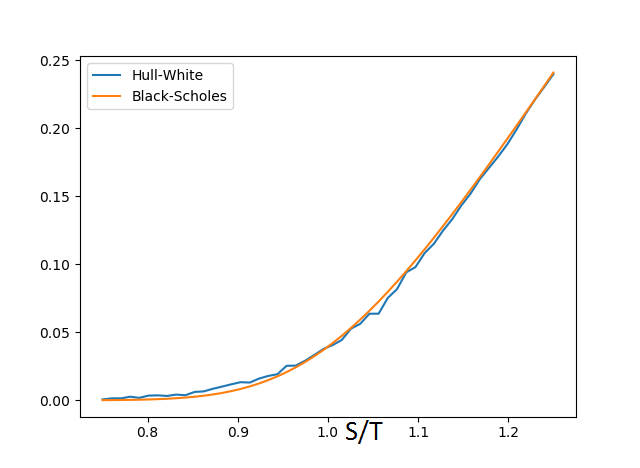
\includegraphics[scale=0.7]{hwrho_0,5.png}
\end{center}
\caption{Ecart relatif du prix par Hull-White par rapport à Black-Scholes (en \%) pour $\rho = 0.5$}
\end{figure}

\begin{figure}[H]
\begin{center}
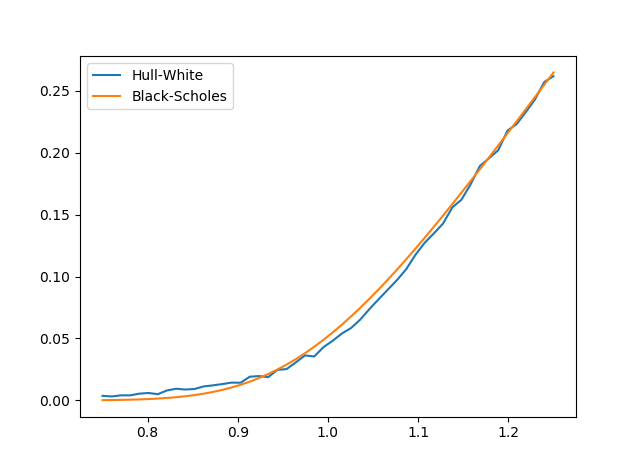
\includegraphics[scale=0.7]{hwrho_0,9.png}
\end{center}
\caption{Ecart relatif du prix par Hull-White par rapport à Black-Scholes (en \%) pour $\rho = 0.9$}
\end{figure} 

On constate que plus la corrélation est élevée entre $V$ et $S$ et plus le pris de Hull-White semble s'éloigner de celui de Black-Scholes. Cela n'est pas étonnant car le prix de Hull-White avec $\rho = 0$ ressemblait beaucoup à celui de black Scholes dans la manière avec laquelle il était obtenu, surtout si la volatilité variait peu autour de $V_0$.

\subsection*{Smile de volatilité:}
Pour déterminer le smile de volatilité, on peut s'inspirer de la dérivation de la volatilité locale proposée par Derman et Kani, qui permet de faire le lien entre valatilité locale (qui nous permet de tracer facilement le smile) et volatilité stochastique (celle dont on dispose et que l'on sait simuler).
\begin{eqnarray*}
V_{Loc}(K, T) = \mathbb{E}\big[V_T | S_T = K]
\end{eqnarray*}
Il nous faut donc calculer l'espérence du la volatilité stochastique conditionnellement à un certain nombre d'état du prix du sous-jacent. On continue à procéder par monte-Carlo, en simulant comme précédemment $N$ évolutions de prix d'actifs ainsi que leur volatilité $\big((S^i_k, V^i_k)_{1\leq k\leq n}\big)_{1\leq i\leq N}$ et en calculant pour des intervalles $I_j = [K_j, K_{j+1}]$ bien choisis:
\begin{eqnarray*}
V_{Loc}\Big(\frac{K_j + K_{j+1}}{2}, T\Big) = \sum\limits_{i=1}^N\frac{V^i_n 1_{\{S^i_n \in I_j\}}}{\sum{1_{\{S^i_n \in I_j\}}}}
\end{eqnarray*}

\begin{figure}[H]
\begin{center}
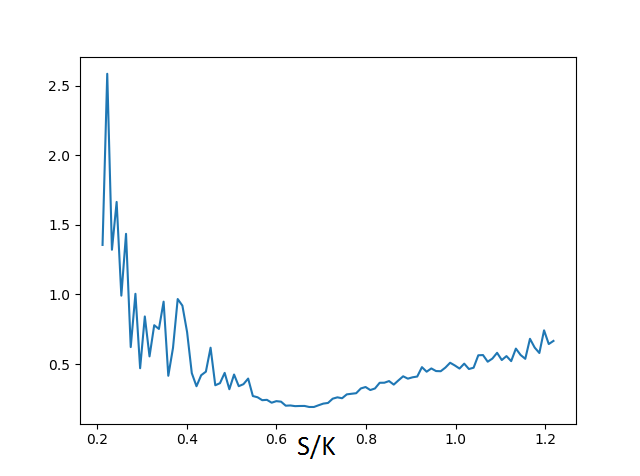
\includegraphics[scale=0.7]{smile01.png}
\end{center}
\caption{Smile de volatilité pour $\rho = 0.9$, $T = 5$}
\end{figure} 

On peut voir que cette méthode a une faiblesse, puisque pour des valeurs extrêmes de $K$ on au moins de données par la simulation que pour les valeurs centrales, et donc l'approximation de l'espérance par Monte-Carlo est moins fiable (et on voit apparaître des oscillations). On peut palier ce problème en rêglant la taille des intervalles (mais en perdant en précision) ou en ajoutant des simulations (en augmentant $N$ et donc forcément le temps de calcul).

\begin{figure}[H]
\begin{center}
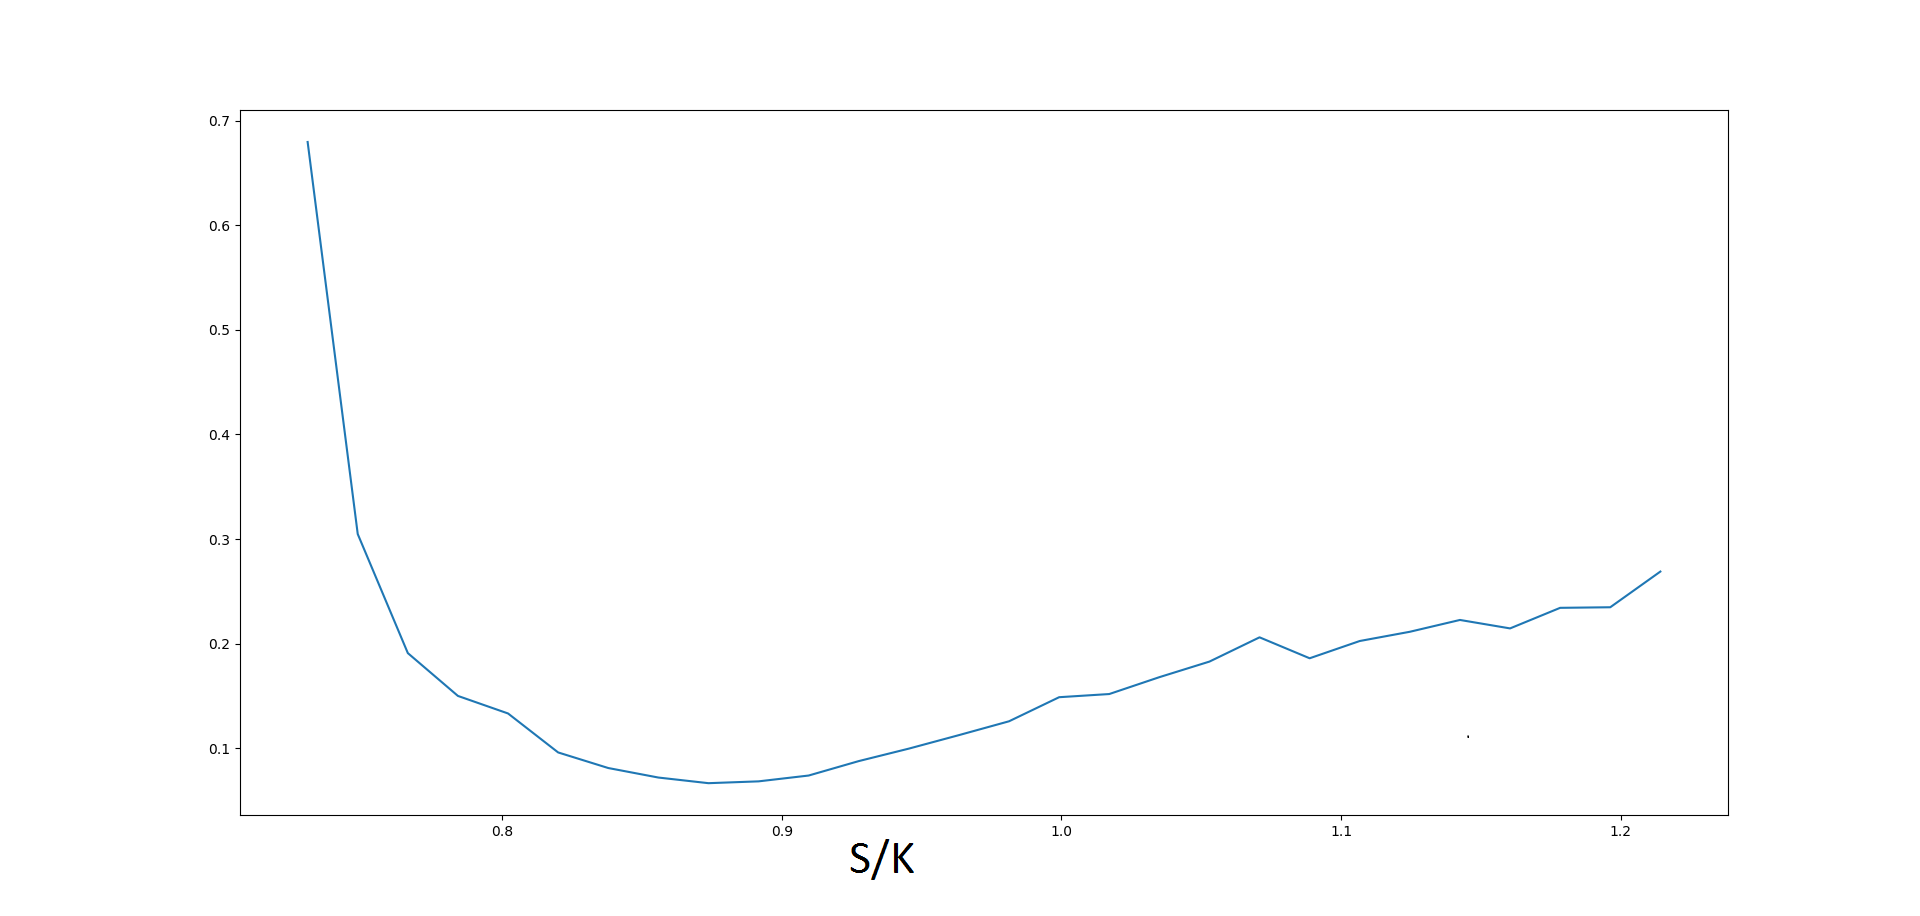
\includegraphics[scale=0.3]{smile02.png}
\end{center}
\caption{Smile de volatilité pour $\rho = 0.9$, $T = 5$}
\end{figure} 
\newpage

\section*{Annexe : Code}
\begin{verbatim}
from math import *
import numpy as np
import matplotlib.pyplot as plt
from scipy.stats import norm
import sys, os

def calcVar(V0, theta, n, mu, xi, a=None):
	dt = theta/n
	nu = np.random.normal(0, 1, n)
	V1 = [V0]
	V2 = [V0]
	change = (a != None)

	for i in range(1, n+1):
		if change:
			mu = a*(np.sqrt(V0) - np.sqrt(V1[i-1]))
		V1 += [V1[i-1]*np.exp((mu - xi*xi/2)*dt + nu[i-1]*xi*np.sqrt(dt))]
		if change:
			mu = a*(np.sqrt(V0) - np.sqrt(V2[i-1]))
		V2 += [V2[i-1]*np.exp((mu - xi*xi/2)*dt - nu[i-1]*xi*np.sqrt(dt))]
	return np.array(V1), np.array(V2)

def BlackScholes(S, K, sigma, theta, r):
	No = norm(0,1)
	d1 = (np.log(S/K) + (r + (sigma*sigma/2))*theta)/(sigma*np.sqrt(theta))
	d2 = d1 - sigma*np.sqrt(theta)
	return S*No.cdf(d1) - K*np.exp(-r*theta)*No.cdf(d2)


def HullWhite1(S, K, sigma0, theta, r, mu, xi, n, N, a=None, rho=None):
	moy = 0
	sigma = 0
	for i in range(N):
		if rho==None:
			V1, V2 = calcVar(sigma0*sigma0, theta, n, mu, xi, a)
			sigma1 = np.sqrt(np.mean(V1))
			sigma2 = np.sqrt(np.mean(V2))
			p1 = BlackScholes(S, K, sigma1, theta, r)
			p2 = BlackScholes(S, K, sigma2, theta, r)
			y = (p1+p2)/2
			moy += y
		else:
			res = calcVarPrice(sigma0*sigma0, S, K, theta, n, r, mu, xi, rho, a)
			moy += res[0]
			sigma += res[1]
	moy = moy/N
	sigma = sigma/N
	return moy, sigma

def curbHW1(sigma0, theta, r, mu, xi, n, N, start=0.75, stop=1.25, step = 0.01, a=None, rho=0):
	beta = start
	tab = []
	l = []
	sig = []
	num = (stop-start)/step
	p_old = 0
	p_new = 0
	while beta < stop:
		res = HullWhite1(beta, 1, sigma0, theta, r, mu, xi, n, N, a, rho)
		tab += [res[0]]
		sig += [res[1]]
		l += [BlackScholes(beta, 1, sigma0, theta, r)]
		beta += step
		p_new = int((beta-start)*100/(stop-start))
		if p_new > p_old:
			p_old = p_new
			if p_new in [10, 20, 30, 40, 50, 60, 70, 80, 90]:
				print(p_new, end='')
				sys.stdout.flush()
			else:
				print('#', end='')
				sys.stdout.flush()
	print('\n')
	prop = np.linspace(start, stop, len(tab))
	plt.figure()
	plt.plot(prop, tab, label = "Hull-White")
	plt.plot(prop, l, label = "Black-Scholes")
	plt.legend()
	plt.show()
	bias = 100*(np.array(tab)-np.array(l))/(np.array(l)+1e-10)
	plt.figure()
	plt.plot(prop, bias)
	plt.show()
	plt.figure()
	plt.plot(prop, sig)
	plt.grid()
	plt.show()
	return prop, tab, l, bias, sig




def calcVarPrice(V0, S0, K, theta, n, r, mu, xi, rho, a=None, final = False):
	S1 = [S0]
	S2 = [S0]
	S3 = [S0]
	S4 = [S0]
	V1 = [V0]
	V2 = [V0]
	V3 = [V0]
	V4 = [V0]
	dt = theta/n
	nu = np.random.normal(0, 1, n)
	u = np.random.normal(0, 1, n)
	for i in range(1, n+1):
		S1 += [S1[i-1]*np.exp((r-V1[i-1]/2)*dt + u[i-1]*np.sqrt(V1[i-1]*dt))]
		V1 += [V1[i-1]*np.exp((mu - xi*xi/2)*dt + rho*u[i-1]*xi*np.sqrt(dt) 
		+ np.sqrt(1 - rho*rho)*nu[i-1]*xi*np.sqrt(dt))]
		S2 += [S2[i-1]*np.exp((r-V2[i-1]/2)*dt - u[i-1]*np.sqrt(V2[i-1]*dt))]
		V2 += [V2[i-1]*np.exp((mu - xi*xi/2)*dt - rho*u[i-1]*xi*np.sqrt(dt) 
		+ np.sqrt(1 - rho*rho)*nu[i-1]*xi*np.sqrt(dt))]
		S3 += [S3[i-1]*np.exp((r-V3[i-1]/2)*dt + u[i-1]*np.sqrt(V3[i-1]*dt))]
		V3 += [V3[i-1]*np.exp((mu - xi*xi/2)*dt + rho*u[i-1]*xi*np.sqrt(dt) 
		- np.sqrt(1 - rho*rho)*nu[i-1]*xi*np.sqrt(dt))]
		S4 += [S4[i-1]*np.exp((r-V4[i-1]/2)*dt - u[i-1]*np.sqrt(V4[i-1]*dt))]
		V4 += [V4[i-1]*np.exp((mu - xi*xi/2)*dt - rho*u[i-1]*xi*np.sqrt(dt) 
		- np.sqrt(1 - rho*rho)*nu[i-1]*xi*np.sqrt(dt))]
	S1 = np.array(S1)
	S2 = np.array(S2)
	S3 = np.array(S3)
	S4 = np.array(S4)
	V1 = np.array(V1)
	V2 = np.array(V2)
	V3 = np.array(V3)
	V4 = np.array(V4)
	p1 = np.exp(-r*theta)*max(S1[n]-K, 0)
	p2 = np.exp(-r*theta)*max(S2[n]-K, 0)
	p3 = np.exp(-r*theta)*max(S3[n]-K, 0)
	p4 = np.exp(-r*theta)*max(S4[n]-K, 0)
	if final:
		sigma1 = V1[n]
		sigma2 = V2[n]
		sigma3 = V3[n]
		sigma4 = V4[n]
		return  (S1[n]+S2[n]+S3[n]+S4[n])/4, (sigma1+sigma2+sigma3+sigma4)/4	
	sigma1 = np.mean(np.sqrt(V1))	
	sigma2 = np.mean(np.sqrt(V2))
	sigma3 = np.mean(np.sqrt(V3))
	sigma4 = np.mean(np.sqrt(V4))
	return (p1+p2+p3+p4)/4, (sigma1+sigma2+sigma3+sigma4)/4


def smile(V0, S0, theta, n, N, r, mu, xi, rho, a=None, num=100, M = None):
	S = []
	V = []
	tab = np.zeros(num) + 1e-10
	E = np.zeros(num)
	p_old = 0
	p_new = 0
	for i in range(N):
		res = calcVarPrice(V0, S0, 1, theta, n, r, mu, xi, rho, a, True)
		S += [res[0]]
		V += [res[1]]
		p_new = int(i*100/N)
		if p_new > p_old:
			p_old = p_new
			if p_new in [10, 20, 30, 40, 50, 60, 70, 80, 90]:
				print(p_new, end='')
				sys.stdout.flush()
			else:
				print('#', end='')
				sys.stdout.flush()
	print('\n')
	S = np.array(S)
	V = np.array(V)
	smin = min(S)
	smax = max(S)
	if M != None:
		smax = min(smax, M)
	stab = np.linspace(smin, smax, num)
	for i in range(N):
		ind = int((S[i]-smin)*(num-1)/(smax-smin))
		if S[i] <= smax:
			tab[ind] += 1
			E[ind] += V[i]
	E = E/tab
	return stab, np.sqrt(E)

#stab1, E1 = smile(0.15*0.15, 1, 5, 50, 10000, 0, 0, 1, 0.9, M=1.25)
#plt.plot(stab1, E1)
#plt.show()
\end{verbatim}
\end{document}